\section{Evietania Charis Sujadi(1174051)}
\subsection{PYSHP Reader}
\begin{enumerate}
    \item Buatlah Script Python dan jelaskan berbaris
    \lstinputlisting[firstline=8, lastline=10]{src/1174051/3/tugas3.py}
    \hfill\break
    \begin{figure}[H]
		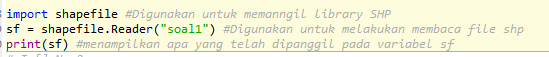
\includegraphics[width=4cm]{figures/1174051/3/1.png}
		\centering
		\caption{Hasil dari SHP Reader Soal 1}
    \end{figure}
    
    \item Buatlah Script Python dan jelaskan
    \lstinputlisting[firstline=12, lastline=14]{src/1174051/3/tugas3.py}
    \hfill\break
    \begin{figure}[H]
		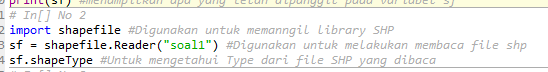
\includegraphics[width=4cm]{figures/1174051/3/2.png}
		\centering
		\caption{Hasil dari SHP Reader Soal 2}
    \end{figure}
    
    \item Buatlah Script Python dan jelaskan perbaris
    \lstinputlisting[firstline=16, lastline=18]{src/1174051/3/tugas3.py}
    \hfill\break
    \begin{figure}[H]
		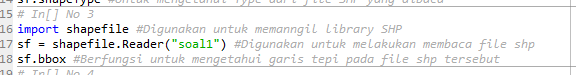
\includegraphics[width=4cm]{figures/1174051/3/3.png}
		\centering
		\caption{Hasil dari SHP Reader Soal 3}
    \end{figure}
    
    \item Buatlah Script Python dan jelaskan perbaris
    \lstinputlisting[firstline=20, lastline=23]{src/1174051/3/tugas3.py}
    \hfill\break
    \begin{figure}[H]
		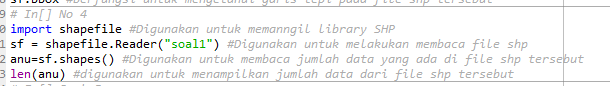
\includegraphics[width=4cm]{figures/1174051/3/4.png}
		\centering
		\caption{Hasil dari SHP Reader Soal 4}
    \end{figure}
    
    \item Buatlah Script Python dan jelaskan perbaris
    \lstinputlisting[firstline=25, lastline=29]{src/1174051/3/tugas3.py}
    \hfill\break
    \begin{figure}[H]
		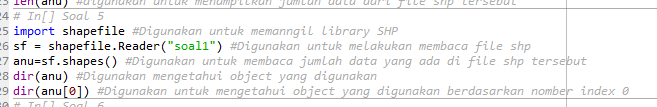
\includegraphics[width=4cm]{figures/1174051/3/5.png}
		\centering
		\caption{Hasi daril SHP Reader Soal 5 Codingan}
    \end{figure}

    \hfill\break
    \begin{figure}[H]
		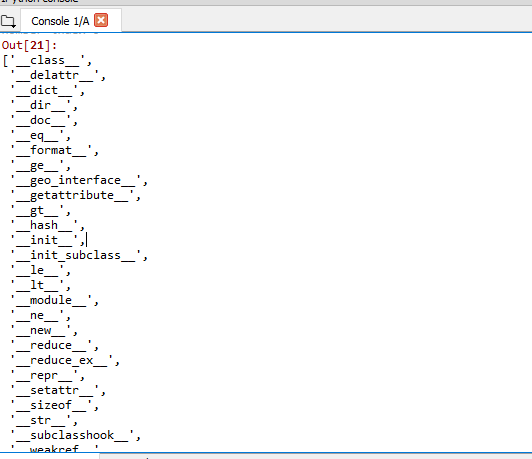
\includegraphics[width=4cm]{figures/1174051/3/5hasil.png}
		\centering
		\caption{Hasil SHP Reader Soal 5 Hasil}
    \end{figure}
    
    \item Buatlah Script Python dan jelaskan perbaris
    \lstinputlisting[firstline=31, lastline=34]{src/1174051/3/tugas3.py}
    \hfill\break
    \begin{figure}[H]
		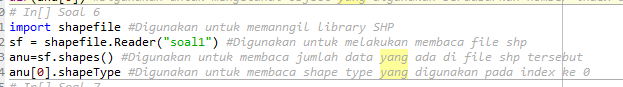
\includegraphics[width=4cm]{figures/1174051/3/6.png}
		\centering
		\caption{Hasil dari SHP Reader Soal 6}
    \end{figure}

    \item Buatlah Script Python dan jelaskan perbaris
    \lstinputlisting[firstline=36, lastline=41]{src/1174051/3/tugas3.py}
    \hfill\break
    \begin{figure}[H]
		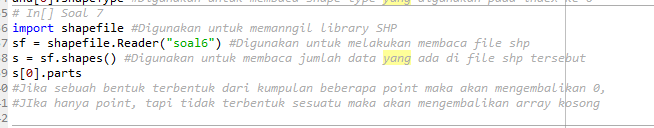
\includegraphics[width=4cm]{figures/1174051/3/7.png}
		\centering
		\caption{Hasi daril SHP Reader Soal 7}
    \end{figure}

    \item Buatlah Script Python dan jelaskan perbaris
    \lstinputlisting[firstline=44, lastline=47]{src/1174051/3/tugas3.py}
    \hfill\break
    \begin{figure}[H]
		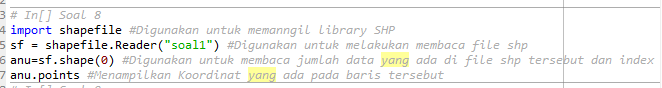
\includegraphics[width=4cm]{figures/1174051/3/8.png}
		\centering
		\caption{Hasil dari SHP Reader Soal 8}
    \end{figure}

    \item Buatlah Script Python dan jelaskan perbaris
    \lstinputlisting[firstline=49, lastline=52]{src/1174051/3/tugas3.py}
    \hfill\break
    \begin{figure}[H]
		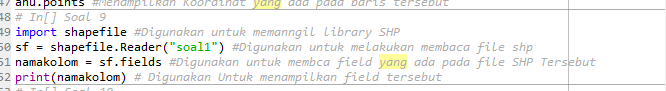
\includegraphics[width=4cm]{figures/1174051/3/9.png}
		\centering
		\caption{Hasil dari SHP Reader Soal 9}
    \end{figure}

    \item Buatlah Script Python dan jelaskan perbaris
    \lstinputlisting[firstline=54, lastline=57]{src/1174051/3/tugas3.py}
    \hfill\break
    \begin{figure}[H]
		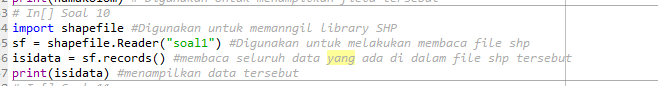
\includegraphics[width=4cm]{figures/1174051/3/10.png}
		\centering
		\caption{Hasil dari SHP Reader Soal 10}
    \end{figure}

    \item Buatlah Script Python dan jelaskan berbaris
    \lstinputlisting[firstline=59, lastline=63]{src/1174051/3/tugas3.py}
    \hfill\break
    \begin{figure}[H]
		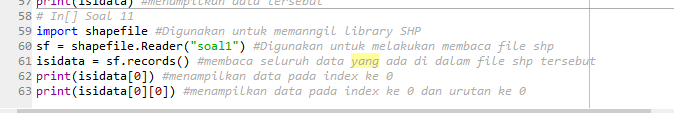
\includegraphics[width=4cm]{figures/1174051/3/11.png}
		\centering
		\caption{Hasil dari SHP Reader Soal 11}
    \end{figure}
\end{enumerate}
\subsection{Link Youtube}
\href{https://youtu.be/TldvcY9GCMA}{Video Youtube}